\documentclass[12pt]{article}
\usepackage[top=1in, bottom=1in, left=1in, right=1in]{geometry}

\usepackage{setspace}
\onehalfspacing

\usepackage{amssymb}
%% The amsthm package provides extended theorem environments
\usepackage{amsthm}
\usepackage{epsfig}
\usepackage{times}
\renewcommand{\ttdefault}{cmtt}
\usepackage{amsmath}
\usepackage{graphicx} % for graphics files
\usepackage{tabu}

% Draw figures yourself
\usepackage{tikz} 

% writing elements
%\usepackage{mhchem}

\usepackage{paralist}

% The float package HAS to load before hyperref
\usepackage{float} % for psuedocode formatting
\usepackage{xspace}

% from Denovo Methods Manual
\usepackage{mathrsfs}
\usepackage[mathcal]{euscript}
\usepackage{color}
\usepackage{array}

\usepackage[pdftex]{hyperref}
\usepackage[parfill]{parskip}

% math syntax
\newcommand{\nth}{n\ensuremath{^{\text{th}}} }
\newcommand{\ve}[1]{\ensuremath{\mathbf{#1}}}
\newcommand{\Macro}{\ensuremath{\Sigma}}
\newcommand{\rvec}{\ensuremath{\vec{r}}}
\newcommand{\vecr}{\ensuremath{\vec{r}}}
\newcommand{\omvec}{\ensuremath{\hat{\Omega}}}
\newcommand{\vOmega}{\ensuremath{\hat{\Omega}}}
\newcommand{\even}{\ensuremath{\phi^g}}
\newcommand{\odd}{\ensuremath{\vartheta^g}}
\newcommand{\evenp}{\ensuremath{\phi^{g'}}}
\newcommand{\oddp}{\ensuremath{\vartheta^{g'}}}
\newcommand{\Sn}{\ensuremath{S_N} }
\newcommand{\Ye}[2]{\ensuremath{Y^e_{#1}(\vOmega_#2)}}
\newcommand{\sigg}[1]{\ensuremath{\Macro^{g'\rightarrow g}_{s,#1}}}
\newcommand{\psig}{\ensuremath{\psi^g}}
%---------------------------------------------------------------------------
%---------------------------------------------------------------------------
\begin{document}
\begin{center}
{\bf NE 155/255, Fall 2019 \\
Discrete Ordinates\\
October 02, 2019}
\end{center}

\setlength{\unitlength}{1in}
\begin{picture}(6,.1) 
\put(0,0) {\line(1,0){6.25}}         
\end{picture}


%---------------------------------------------------------------------------
%---------------------------------------------------------------------------
\section*{Angular Discretization, Continued}

Recall this substitution in order to satisfy the orthogonality 
requirement:

\begin{equation}
\hat{Y}^e_{lm} = \frac{1}{\sqrt{2-\delta_{m0}}}Y^e_{lm}\:,\quad
\hat{Y}^o_{lm} = \frac{1}{\sqrt{2-\delta_{m0}}}Y^o_{lm}\:.
\end{equation}

Because \(\hat{Y}_{\ell0}^o=0\) based on the inclusion of \(\sin(m\varphi)\) in 
its definition, the above sometimes neglects the \(\delta_{m0}\) term in the 
odd function since it is implied that \(m=0\) leads to an identically zero 
function anyways.

Next, we expand the Spherical Harmonics into real and imaginary components. 
The sum over $m>0$ then becomes 

\begin{equation}
\sum_{m=1}^l\Bigl(
\hat{Y}^e_{\ell m}(\vOmega)\hat{Y}^e_{\ell m}(\vOmega') +
\hat{Y}^o_{\ell m}(\vOmega)\hat{Y}^o_{\ell m}(\vOmega') +
\hat{Y}^e_{\ell-m}(\vOmega)\hat{Y}^e_{\ell-m}(\vOmega') +
\hat{Y}^o_{\ell-m}(\vOmega)\hat{Y}^o_{\ell-m}(\vOmega')\Bigr)\:,
\end{equation}
where the imaginary terms have been set to zero because our values must be
real. 

Next, we use these relationships to get rid of the $-m$ terms:

\begin{align}
 \hat{Y}^e_{\ell-m} &= (-1)^{-m}\hat{Y}^e_{\ell m} \equiv
 (-1)^m\hat{Y}^e_{\ell m} \:\text{ and}\\
 \hat{Y}^o_{\ell-m} &= -(-1)^m\hat{Y}^o_{\ell m}\:,
\end{align}

and then the summation becomes

\begin{equation}
  \sum_{m=1}^l\Bigl(
  2\hat{Y}^e_{\ell m}(\vOmega)\hat{Y}^e_{\ell m}(\vOmega') +
  2\hat{Y}^o_{\ell m}(\vOmega)\hat{Y}^o_{\ell m}(\vOmega')\Bigr).
\end{equation}

After applying these equations in the $m>0$ terms and combining with the $m=0$
term described above, the expression for $P_\ell(\vOmega\cdot\vOmega')$ is
\begin{equation}
  P_\ell(\vOmega'\cdot\vOmega) = \frac{4\pi}{2\ell+1}
  \Bigl[
  Y^e_{\ell0}(\vOmega)Y^e_{\ell0}(\vOmega') +
  \sum_{m=1}^\ell
  \bigl(Y^e_{\ell m}(\vOmega)Y^e_{\ell m}(\vOmega') +
  Y^o_{\ell m}(\vOmega)Y^o_{\ell m}(\vOmega')\bigr)\Bigr]\:.
    \label{eq:P_l(mu_o)}
\end{equation}

Here we have replaced the $\hat{Y}$ terms with their respective definitions
so that we are once again working in terms of regular spherical harmonics.

\subsubsection*{Representing Sources with Spherical Harmonics}

We can use these terms to expand our scattering and external sources (adding 
energy indexing back in) for multi-D and any degree of anisotropy. We define
the \textbf{scattering source} as:

\begin{align}
Q^g_{s}(\vec{r},\vOmega) &=
\sum_{g'=0}^{G-1} \sum_{\ell=0}^{N} \frac{2\ell+1}{4 \pi} \Sigma^{g'\rightarrow g}_{s,\ell}(\vecr)
\int_{4\pi} d\vOmega'\: P_\ell(\vOmega \cdot \vOmega') \psi^{g'}(\vecr, \vOmega')\\
  Q^g_{s}(\vec{r},\vOmega) &= \sum_{g'=0}^{G-1}
  \sum_{\ell=0}^N
  \sigg{\ell}(\vec{r})
  \Bigl[
  Y^e_{\ell0}(\vOmega)\evenp_{\ell0}(\vec{r}) +
  \sum_{m=1}^\ell
  \bigl(
  Y^e_{\ell m}(\vOmega)\evenp_{\ell m}(\vec{r}) +
  Y^o_{\ell m}(\vOmega)\oddp_{\ell m}(\vec{r})
  \bigr)\Bigr]\:,
  \label{eq:mg-scattering-source}
\end{align}
where
\begin{alignat}{3}
  \even_{\ell m} &= \int_{4\pi}Y^e_{\ell m}(\vOmega)\psi^g(\vOmega)\:d\vOmega\:,
  \quad& m\ge 0\:,\label{eq:even-flux}\\
  %%
  \odd_{\ell m} &= \int_{4\pi}Y^o_{\ell m}(\vOmega)\psi^g(\vOmega)\:d\vOmega\:,
  \quad& m>0\:.\label{eq:odd-flux}
\end{alignat}

Equation~(\ref{eq:mg-scattering-source}) is the multigroup anisotropic
scattering source that is defined by the order of the Legendre expansion,
$P_N$, of the scattering.  For a given $P_N$ order, $(N+1)^2$ moments are
required to integrate the scattering operator.  The moments in
Eqs.~(\ref{eq:even-flux}) and (\ref{eq:odd-flux}) are the \textit{angular flux 
moments} or, simply, flux moments.
  
Applying the same methodology gives the expansion of the \textbf{external 
source}:

\begin{equation}
  Q^g_e(\vec{r}, \vOmega) = \sum_{\ell=0}^{N}\Bigl[
  Y^e_{\ell0}(\vOmega)q^g_{\ell0}(\vec{r}) +
  \sum_{m=1}^{\ell}
  \bigr(
  Y^e_{\ell m}(\vOmega)q^g_{\ell m}(\vec{r}) + Y^o_{\ell m}(\vOmega)s^g_{\ell m}(\vec{r})\bigr)
  \Bigr]\:,
  \label{eq:mg-external-source}
\end{equation}

where the spatial dependence has been suppressed.  The even and odd source
moments are defined as

\begin{alignat}{3}
  q^g_{\ell m} &= \int_{4\pi}Y^e_{\ell m}(\vOmega)q^g_e(\vOmega)\:d\vOmega\:,
  \quad&m\ge 0\:,\label{eq:even-source}\\
  s^g_{\ell m} &= \int_{4\pi}Y^o_{\ell m}(\vOmega)q^g_o(\vOmega)\:d\vOmega\:,
  \quad&m>0\:.\label{eq:odd-source}
\end{alignat}

\subsubsection*{Discrete Ordinates Equations}

We put all of that together to get

\begin{align*}
\vOmega_a \cdot \nabla \psi^g_a(\vecr) &+ \Sigma^g_t(\vecr)\psi^g_a(\vecr) = \\
&\sum_{g'=0}^{G-1}
  \sum_{\ell=0}^N
  \sigg{\ell}(\vec{r})
  \Bigl[
  Y^e_{l0}(\vOmega)\evenp_{\ell0}(\vec{r}) +
  \sum_{m=1}^\ell
  \bigl(
  Y^e_{\ell m}(\vOmega)\evenp_{\ell m}(\vec{r}) +
  Y^o_{\ell m}(\vOmega)\oddp_{\ell m}(\vec{r})
  \bigr)\Bigr]\\
&+\sum_{\ell=0}^{N}\Bigl[
  Y^e_{\ell0}(\vOmega)q^g_{\ell0}(\vec{r}) +
  \sum_{m=1}^{\ell}
  \bigr(
  Y^e_{\ell m}(\vOmega)q^g_{\ell m}(\vec{r}) + Y^o_{\ell m}(\vOmega)s^g_{\ell m}(\vec{r})\bigr)
  \Bigr]
\end{align*}

The $S_N$ method will be conservative if the quadrature set effectively
integrates the even and odd Spherical Harmonics.

The thing that you solve for is the flux moments, and then you reconstruct 
that flux at the end.

\subsubsection*{Azimuthal Symmetry}

This all gets simpler if we have azimuthal symmetry. In that case, $m=0$ and 

\[
  Y_{\ell0}(\theta,\varphi) = (-1)^0\sqrt
  {
    \frac{2\ell+1}{4\pi}\frac{(\ell-0)!}{(\ell+0)!}
  }\,
  P_{\ell0}(\cos\theta)\mathrm{e}^{i0\varphi} =
  \sqrt{\frac{2\ell+1}{4\pi}}P_{\ell}(\cos\theta),
\]

then

\begin{align*}
\vOmega_a \cdot \nabla \psi^g_a(\vecr) &+ \Sigma^g_t(\vecr)\psi^g_a(\vecr)  \\
&=\sum_{g'=0}^G
  \sum_{\ell=0}^N
  \sigg{\ell}(\vec{r})
  \bigl(
  Y^e_{\ell}(\vOmega) \evenp_{\ell}(\vec{r}) \bigr)
+\sum_{\ell=0}^{N}\bigl(
  Y^e_{\ell}(\vOmega)q^g_{\ell}(\vecr)\bigr)\\
  %
 &=\sum_{g'=0}^G
  \sum_{\ell=0}^N \sigg{\ell}(\vec{r})
  \bigg[\sqrt{\frac{2\ell+1}{4\pi}}P_{\ell}(\cos\theta)\evenp_{\ell}(\vec{r}) \bigg]
  + \sum_{l=0}^{N}
  \bigg[\sqrt{\frac{2\ell+1}{4\pi}}P_{\ell}(\cos\theta)q^g_{\ell}(\vecr)\bigg]
\end{align*}

which is equivalent to what we did in the simplification class.

%-----------------------------------------
\subsubsection*{Discrete Ordinates Considerations}

Two main things to consider in discrete ordinates: \textit{quadrature choice} 
and \textit{ray effects}. 

\textbf{Level-symmetric} quadratures use the same set of $N/2$ positive values 
of direction cosines with respect to each of the three axes. That is, for each 
level $n$ we set $\mu_a = \eta_a = \xi_a$. We describe a level $a$ as the 
ordinate set that has cosine $\mu_a$ with respect to the $x$-axis. Note that 
with this setup no axis has preferential treatment. \autoref{fig:levelsym} 
shows $S_6$. We see there are $6/2 = 3$ values of each direction cosine, and 
each one is the same with respect to each axis. We have $N(N+2)$ quadrature
points over the sphere, and that divided by 8 per octant (in this case 48 and
6, respectively). 

\begin{figure}[h!]
    \begin{center}
    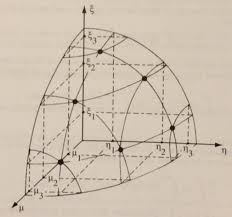
\includegraphics[keepaspectratio, width = 2.5 in]{level-sym}
    \end{center}
    \caption{$S_6$ quadrature}
    \label{fig:levelsym}
\end{figure}

Because of the symmetry constraints, not all of the $\mu_n$ are independent. In 
fact, there is only one degree of freedom because of all of the constraints. 
Choosing $\mu_1$ sets all of the other values as follows:

\[
\mu_i^2 = \mu_1^2 + \frac{2(1 - 3\mu_1^2)}{N-2}(i-1)\:.
\]

See 4-2 of Lewis and Miller for details. Selecting a $\mu_1$ near the poles 
will cause clustering at the poles, and so on. 

Further, we need to select weights to perform the integration. These meet the 
requirement

\[
\sum_{a=1}^{N(N+2)/8} w_a = 1\:.
\]

In the $S_2$ approximation, we only have one choice. For higher values we 
still have some choices. 

A common choice is to choose weights and angles that correctly integrate as 
many Legendre Polynomials as possible. These are shown in in Table 4-1 in L\&M 
and are technically called the $LQ_N$ set. There are other $S_N$ versions that 
have reduced symmetry or relaxation of requirements in other ways. For 
example, if we don't require all of the cosines to lie on the $N/2$ levels we 
can maintain rotational symmetry and have equal weights. 

\end{document}
